\documentclass{standalone}
\begin{document}
As discussed in Chapter~\ref{chap:intro}, a significant caveat when using classical simulations to study quantum speedup is that the complexity of a simulation in a given framework does not exclude a more efficient description in an alternative picture. While in general for a system with arbitrary states and arbitrary operations, no efficient classical implementation should exist under the Church-Turing-Deutsch thesis~\cite{Deutsch1985}, the computational complexity of different quantum computing methods is nonetheless instructive to consider. 
\par
A significant example of this is the development of a novel technique we will call \texttt{BGSS} or the `Stabiliser Rank' method, for simulating Clifford+T quantum circuits developed in a pair of papers by Bravyi, Gosset, Smolin \& Smith~\cite{Bravyi2015,Bravyi2016b}. In particular, this algorithm is capable of sampling the output distribution of a computation made up of $m$ gates on $n$ qubits and $t$ T gates in a time that scales as $O(2^{0.23t}t^{3})$~\cite{Bravyi2016b}. This represents a significant in computational complexity over the \texttt{CHP} method of Aaronson \& Gottesman, which scales as $O(2^{4t})$~\cite{Aaronson2004a}.
\par
The core of this \texttt{BSSG} algorithm lies in two results. The first is that any circuit on $n$ qubits with $t$ T-gates can be rewritten as a sequence of Pauli measurements acting on $t$ edge-type magic states. This is a new model of quantum computation called a `Pauli Based Computation'(PBC)~\cite{Bravyi2015}. 
\par
The second result is that it is possible to find decompositions of $n$ qubit states states into a sum of non-orthogonal $n$ qubit stabilizer states. The number if states in this decomposition is called the Stabiliser rank $\chi$, and $\chi\leq2^{\frac{n}{2}}$ for edge-type magic states~\cite{Bravyi2016b,Bravyi2015}.
\par
In this Chapter, we discuss the proof of these two techniques, and in particular focus on proving the asymptotic limit for the Stabiliser rank of the edge type magic states. We then discuss the algorithmic implementation of the method, and it's significance for quantum computation. 

\section{Pauli Based Computation}\label{sec:pbc}
A PBC is defined by a sequence of $m$ Pauli measurements on $t$ qubits $P_{i}:i\in\{1,2,\cdots,m\}$. As these are Pauli measurements, at each step we obtain an outcome $\sigma_{i}=\pm 1$. We allow the choice of Pauli operator to be `adaptive', such that the measurement performed at step $j$ can depend on all the previous outcomes $\{\sigma_{1},\cdots,\sigma_{j-1}$. The final sequence of measurement outcomes is then processed classically to give the result of the computation. 
\par
Bravyi, Smolin and Smith showed that, if the $t$ qubits used in the computation are initialised as the magic state $\ket{A}$, then a PBC is capable of simulating a Clifford+T circuit with $t$ T-gates. The other components of the circuit determine the sequence of Pauli measurements~\cite{Bravyi2015}. 
\par
We can begin to understand this correspondence by defining a looser model called a PBC*, where a subset of the qubits in the computation are initialised in the computational state $\ket{0}$, and the rest are initialised as magic states $\ket{A}$. We consider a computation $U$, made up of $c$ Clifford and $t$ T gates on $n$ qubits, followed by a measurement in the computational basis. We can convert this to something resembling a PBC* by replacing each $T$ gate with a magic state injection gadget, as shown in Fig.~\ref{fig:MSI}. 
\par
We thus define the new `gadgetized' circuit $V$ acting on $n+t$ qubits, which is made up of only Clifford gates, $X$ basis measurements in the magic state gadgets and a final $Z$ basis measurement on $n$ qubits. As the Clifford group only permutes operators in the Pauli group, we can thus commute the entire circuit $V$ to the end of the computation, after the final measurement, and discard these gates, updating the measurement operators accordingly~\cite{Bravyi2015}. 
\par
Because of the measurement-controlled correction in the magic state gadgets, the resulting Pauli measurements on the computational states will be adaptive. This gives a sequence of $t$ 1-qubit measurements, followed by a readout measurement on $n$ qubits; we have successfully converted the computation to PBC* form. 
\par
We can assume without loss of generality that all these Pauli operators pairwise commute~\cite{Bravyi2015}. To understand why, consider step $q$, which anticommutes with a previous measurement $P_{p}$. Writing the state of the system after the $q-1$ measurements as $\ket{\phi}$, the state obtained after measurement $q$ is $\frac{1}{\sqrt{2}}(\mathbb{I}+\sigma_{q}P_{q})\ket{\phi}$.
\par
We can rewrite this projector as $W_{q}=\frac{1}{\sqrt{2}}(\sigma_{q}P_{q}+\sigma_{p}P_{p})$. For an anticommuting pair of operators $P_{q},P_{p}$, the resulting operator $W\in\mathcal{C}_{2}$, and thus it suffices to pick $\sigma_{t}$ at random, commute the resulting $W_{q}$ to the end of the circuit, and discard it.
\par
We can use this method to prove that the action of the measurements on the qubits initialised in the $\ket{0}$ is trivial~\cite{Bravyi2015}. If we prepend the measurement sequence with computational basis measurements on these $\ket{0}$ qubits, which all have a deterministic outcome $+1$. We can use the above argument to make these measurements commute with the sequence $P_{i}$, such that all these Pauli measurements act trivially on these $n$ qubits. Thus, we can discard them, and obtain a PBC on $t$ qubits~\cite{Bravyi2015}. 

\subsubsection*{Finding the PBC Projector}\label{sec:pbcproj}
We can use this PBC formalism to obtain an explicit form for the probability $P_{out}(x)$ of obtaining a given output string $x$ from the set of all $w$-bit binary strings $\mathbb{Z}_{2}^{w}$, where $w\leq n$. The projector on to this output is given by $\Pi_{x} = \ketbra{x}{x}\otimes\mathbb{I}_{else}$. To simplify the analysis, we can postselect on the measurement outcome of the magic state gadgets, such that we don't have to introduce any correction operations. To compensate, we normalise the probabilities accordingly~\cite{Bravyi2015}. This gives the expression
\begin{equation}
P_{out}(x) = 2^{t}\matrixel{0^{\otimes n}A^{\otimes t}}{V^{\dagger}\left(\Pi_{x}\otimes\ketbra{0^{\otimes t}}{0^{\otimes t}}\right)V}{0^{\otimes n}A^{\otimes t}}
\end{equation}
where $V$ is the circuit including magic state gadgets on the $n+t$ qubits. The projector $\Pi_{x}\otimes\ketbra{0^{\otimes t}}{0^{\otimes t}}\equiv\Pi$, is a projector on to a stabiliser group $\mathcal{W}\subseteq\mathcal{P}_{n+t}$, generated by $-1^{x_{i}}Z_{i}$ for the $i$th bit of the output string, $Z_{j}$ for the $j$th magic state ancilla, and $I$ otherwise.
\par
The action of the Clifford circuit $V$ is thus to map us to a new stabiliser group $\mathcal{V}$ of dimension $w+t$. For any element of $\mathcal{V}$, if the stabiliser doesn't act as $I$ or $Z$ on the first $n$ qubits, then this term reduces to $0$ as 
\[\matrixel{0}{\text{X}}{0}=\matrixel{0}{\text{Y}}{0}=0.\]
Thus, the matrix element is non-zero only on a subset $\mathcal{V}_{0}$ with dimension $v=\vert\mathcal{V}_{0}\vert$, and thus we can write
\begin{equation}
    \matrixel{0^{\otimes n}}{\Pi_{\mathcal{V}}}{0^{\otimes n}} = 2^{-w-t+v}\matrixel{0^{\otimes n}}{\Pi_{\mathcal{V}_{0}}}{0^{\otimes n}}.
\end{equation}
Evaluating the matrix element for the $\ket{0^{\otimes n}}$ states gives a reduced $t$ qubit Stabiliser group $\Pi_{\mathcal{G}}$ acting on the magic states. Taken all together, we thus have 
\begin{equation}
    P_{out}(x) = 2^{v-w}\matrixel{A^{\otimes t}}{\Pi_{G}}{A^{\otimes t}}
\end{equation}
where $\Pi_{G}=\matrixel{0^{\otimes n}}{V^{\dagger}\Pi V}{0^{\otimes n}}$. 

\section{The Stabiliser Rank}\label{sec:srank}
Having proven this alternate form for a Clifford+T circuit, Bravyi, Gosset, Smolin \& Smith then examined the problem of trying to efficiently simulate the PBC. In particular, they use the observation that a Pauli measurement on a Stabiliser state can be simulated in a computational time that scales as $O(n^{3})$~\cite{Aaronson2004a,Bravyi2015}. 
\par
We could then use this observation to try and simulate Pauli measurements on arbitrary states by decomposing them into a mixture of Stabiliser states 
\begin{equation}
\ket{\psi} = \sum_{i=1}^{\chi}z_{i}\ket{\phi_{i}}\quad:\exists\mathcal{S}_{\phi_i}
\end{equation}
We can calculate the matrix element $\matrixel{\phi_{i}}{\Pi_{G}}{\phi_{i}}$ efficiently for each Stabiliser state, and then combine them according to the amplitudes $z_{i}$. The computational complexity of this then scales as $O(\chi\;\poly(n))$, where $\chi$ is called the `Stabiliser Rank' of the state, the number of terms in the decomposition. Stabiliser states also have the obvious property that $\chi=1$, and $\chi$ for an arbitrary $n$ qubit state has a simple upper bound of $2^{n}$, which corresponds to decomposing the state into the computational basis. But, certain states also have a significantly smaller stabiliser rank.
\par
In particular, Bravyi, Smolin \& Smith noted that the Stabiliser rank for $\ket{H}\otimes\ket{H}$\footnote{Recall that the state $\ket{H}$ is equivalent to the magic state $\ket{A}$ to within a Clifford rotation.} is $2$; equal to the rank of an arbitrary single qubit state. This immediately constrains $\chi\leq 2^{\frac{n}{2}}$ for $n$ edge-type magic states, by splitting the state into tensor products of pairs~\cite{Bravyi2015}. Numerical estimates on up to 6 magic states showed that the Stabiliser rank grew slowly, approximately linearly, in the number of copies, and a later analytical effort by Bravyi \& Gosset gave an asymptotic scaling $\chi(\ket{H}^{\otimes t})=O(2^{0.23 t})$~\cite{Bravyi2016b}.
\par
\begin{table}[h]
\centering
\begin{tabular}{||l|r|r|r|r|r|r||}
\hline
$\ket{H^{\otimes n}}$ & 1 & 2 & 3 & 4 & 5 & 6 \\ \hline
$\chi$ & 2 & 2 & 3 & 4 & 6 & 7\\ \hline
\end{tabular}
\caption{Table showing slow growth in the Stabiliser rank for $n$ copies of the magic state, as found in~\cite{Bravyi2015}. These values are estimates, as they were dervied by using Simulated Annealing to search for potential decompositions. In general, finding the Stabiliser rank is computationally demanding as no known algorithm beyond brute-force searching exists.}
\label{tab:approxchi}
\end{table}
An important distinction in this method is that the stabilizer states in the decomposition do not have to be mutually orthogonal. This was a requirement in the extension of \texttt{CHP} to magic states developed by Aaronson \& Gottesman~\cite{Aaronson2004a,Garcia2012}. An alternative idea called `Stabiliser Frame' decomposition was developed by Garcia et al., which built decompositions out of pairs of orthogonal stabiliser states~\cite{Garcia2012,Garcia2015}. The authors successfully demonstrated that this method can achieve a `frame rank' $\vert\mathcal{F}\vert < 2^{k}$. Using this method, they were able to simulate modular exponentiation circuits, which also form a subroutine in Shor's algorithm, achieving a $\vert\mathcal{F}\vert=64$ for a simulation on $5$ logical qubits encoded in an error correction code~\cite{Garcia2015}. However, they did not examine decompositions of magic states, and the pairwise frame construction means this was based on a simulation of $2\times\vert\mathcal{F}\vert$ stabiliser states.
\par
An alternative attempt to find a classical simulation of a Clifford+T simulation was based on the `Discrete Wigner function' quasi-probability formalism, which allows efficient simulation for an state where the distribution is strictly positive valued~\cite{Veitch2012,Howard2014}. It was show that these can be extended to simulate general quantum circuits if they are combined with random sampling techniques, with a resulting running time exponential in the negativity of the Wigner function~\cite{Bravyi2015,Pashayan2015}. Extending this to Clifford+T circuits allows a simulation of a `restricted' PBC made up of only Pauli X and Z measurements, with a complexity $O(2^{0.543 t}\poly(n))$~\cite{Bravyi2015,Delfosse2015}. This is a similar scaling to the `stabiliser rank' method, but importantly this restricted PBC is \emph{not} capable of simulating universal quantum computation~\cite{Bravyi2015}.
\par
Bravyi, Smolin \& Smith also make the following conjecture about the magnitude of the stabiliser rank.
\par
\begin{conj}\label{thm:magicrank}
    For a given state $\ket{\phi}$
    \[\chi_{\phi} 
        \begin{cases}
            = 1 & \text{if } \ket{\phi} \text{ is a stabiliser states} \\
            = \chi_{n} & \text{if } \ket{\phi} \text{ is a magic state} \\
            > \chi_{n} & \text{otherwise} \\
        \end{cases}
    \]
    where $\chi_{n}$ is the small stabiliser rank decomposition for an $n$-qubit magic state.
\end{conj}

In particular, this means that a Clifford+`Magic State' computation seems to be the easiest model to simulate classically. This scaling is still exponential, but the growth of the computational description is smaller than for arbitrary quantum states~\cite{Bravyi2015}. 
\subsection{Bounding $\chi$ for Edge States}\label{sec:edgebound}
The computational complexity of simulating a PBC on stabiliser states is dominated by the scaling of the stabiliser rank $\chi$. In their 2016 paper building on the results of Bravyi, Smolin \& Smith, Bravyi \& Gosset sought an analytical form that would allow them to bound $\chi$ for the edge-type states. Importantly, they also allowed for the possibility of $\delta$-approximate decompositions, such that $\vert\braket{\psi}{H}\vert^{2}\geq 1-\delta$. 
\par
The edge-type state $\ket{H}$ is an eigenstate of the Hadamard operator, and is given by the projection onto the surface of the Bloch sphere of the midpoint along the edge of the set of simulable states connecting $\ket{0}$ and $\ket{+}$, as shown in Fig~\ref{fig:octohedron}. As a result, the state has equal overlap with these two states 
\[\braket{0}{H}=\braket{+}{H}=\cos\left(\frac{\pi}{8}\right)\equiv \nu.\]
This means these two stabiliser states can form a `basis' for the $\ket{H}$ state. Writing $\ket{\tilde{0}}=\ket{0},\ket{\tilde{1}}=\ket{+}$, we can then write the state as a sum over binary strings in this basis
\begin{equation}
  \label{eq:hstrings}
  \ket{H^{\otimes m}}=\frac{1}{(2\nu)^{t}}\sum_{x\in\mathbb{F}_{2}^{n}}\ket{\tilde{x}_{1}\otimes\cdots\otimes\tilde{x}_{t}}
\end{equation}
where $\mathbb{F}_{2}^{t}$ is a finite field, equivalent to the set of $t$-bit binary strings~\cite{Bravyi2016b}. Each of the terms in this decomposition is a tensor product of Stabiliser states, and so is itself a stabiliser state. This decomposition then has a maximal stabiliser rank of $2^{t}$ for $t$-qubits. 
\par
The authors thus consider finding $k$-dimensional linear subspaces of $t$-bit strings, $\mathcal{L}\subseteq\mathbb{F}_{2}^{t}$. This can be understood is a subset of $2^{k}$ strings, such that the combination of any pair of strings in the set under addition (modulo 2) is also in the set. For each of these subspaces, we define an associated normalised state~\cite{Bravyi2016b} 
\begin{equation}
  \label{eq:Hsubspaces}
  \ket{\mathcal{L}}=\frac{1}{\sqrt{2^{k}Z(\mathcal{L})}}\sum_{x\in\mathcal{L}}\ket{\tilde{x}_{1}\otimes\cdots\otimes\tilde{x}_{t}}
\end{equation}
where $Z(\mathcal{L})$ is a `partition function' based on the Hamming weight of each string $\vert x\vert$ that ensures proper normalisation, given by
\begin{equation}
  \label{eq:ZH}
  Z(\mathcal{L})\equiv\sum_{x\in\mathcal{L}}2^{-\frac{\vert x \vert}{2}}.
\end{equation}
Each of these normalised states has a stabiliser rank $2^{k}$, and so the problem now reduces to understanding how small $k$ can be to find a subspace capable of $\delta$ approximating $\ket{H^{\otimes t}}$.
\par
From the overlap with each basis state, we can show that the overlap of the magic states with a subspace $\ket{\mathcal{L}}$ is given by
\begin{equation}
    \label{eq:HLoverlap}
    \vert\braket{H^{\otimes t}}{\mathcal{L}}\vert^{2}=\frac{2^{k}\nu^{2t}}{Z(\mathcal{L})}
\end{equation}
which, as $Z(\mathcal{L})\geq 1$ gives a bound $2^{k}\geq \frac{1}{\nu^{2t}}(1-\delta)$ for a $\delta$ approximate subspace. This can be reined to give the previously stated result
\begin{equation}
2^{k}=O(\nu^{-2t}\delta^{-1})=O(2^{\gamma t}\delta^{-1}),
\end{equation} 
where the value $\gamma=0.23$ comes from rearranging the two expressions to give $\gamma=-2\log_{2}(\vert\braket{\tilde{x}}{H}\vert)$.
\par
To find this bound, we need to bound the value of the partition function $Z(\mathcal{L})$ for an arbitrary subspace.
\par
\begin{lem}\label{thm:expectation}
    Let $\mathcal{L}\subseteq\mathbb{F}_{2}^{t}$ be a $k$ dimensional subspace chosen uniformly at random. Then the expectation value of the partition function $\mathbb{E}(Z(\mathcal{L}))\leq 1+2^{k}\nu^{2t}$.
\end{lem}
\begin{proof}\footnote{The proof described here is as presented in~\cite{Bravyi2016b}. The argument will be given in more detail in section~\ref{sec:frank}.}
    $Z = \sum_{x\in\mathcal{L}}f(x),\;f(x)\equiv 2^{-\frac{\vert x\vert}{2}},\; f(00\cdots 0)=1$. Thus, we can write
    \[\mathbb{E}(Z(\mathcal{L})) = 1+\sum_{x\in\mathbb{F}_{2}^{t}\setminus 0^{t}}f(x)\cdot \mathbb{E}\left(\chi_{\mathcal{L}(x)}\right)\]
    where $\chi_{\mathcal{L}}(x)$ is the `indicator function', which returns $1$ if $x\in\mathcal{L}$ and $0$ otherwise. \\
    We can thus show that
    \begin{align*}
        \mathbb{E}\left(Z(\mathcal{L})\right) 
        &= 1+\frac{2^k-1}{2^t-1}\sum_{x\in\mathbb{F}_{2}^{t}\setminus 0}2^{-\frac{\vert x\vert}{2}}\\
        &=1+\frac{2^k-1}{2^t-1}\left(2^t\nu^{2t}-1\right)\\
        &\leq 1+2^{k}\nu^{2t}\\
    \end{align*}
\end{proof}
\begin{cor}
There exists at least one subspace $\mathcal{L}$ such that it's partition function $Z(\mathcal{L})\leq1+2^{k}\nu^{2t}$.
\end{cor}
Using Markov's inequality, and fixing $k: 4\geq 2^{k}\nu^{2t}\delta\geq 2$, we can show that
\begin{align}\label{eq:markovineq}
\begin{split}
\text{Pr}[\frac{Z(\mathcal{L})}{(1+2^{k}\nu^{2t})(1+\frac{\delta}{2})}\geq 1] 
&\leq \frac{\mathbb{E}(Z(\mathcal{L}))}{(1+2^{k}\nu^{2t})(1+\frac{\delta}{2})} \\
&\leq 1-\frac{\delta}{2+\delta}.
\end{split}
\end{align}
This means that, by picking $O(\frac{1}{\delta})$ subpsaces at random, we can find $\mathcal{L}^{\star}$ such that
\begin{equation}
    Z(\mathcal{L}) \leq (1+2^{k}\nu^{2t})(1+\frac{\delta}{2})
\end{equation}
which, by plugging in to Eq.~\ref{eq:HLoverlap}, gives us the result
\begin{equation}
    \vert\braket{H^{\otimes t}}{\mathcal{L}^{\star}}\vert^{2}\geq 1-\delta.
\end{equation}
Thus, we can find a subspace capable of $\delta$-approximating $\ket{H^{\otimes t}}$ with $2^{k}$ elements that satisfies the above requirement on $k$. This allows us to write $\chi = 2^{k} \leq 4\nu^{-2t}\delta^{-1}$, and obtain the asymptotic bound stated before.
\par
It is important to note that this is an approximate decomposition, and so it's worth asking how this would compare to an approximate decomposition in to computational basis states. Using an argument from information theory, it is clear that the amplitude of $t$ copies of a state $\alpha\ket{0}+\beta\ket{1}$ is concentrated on the `typical' strings with Hamming weight~\cite{Bravyi2016b,Preskill2016}
\begin{equation}\label{eq:hweight}
    \vert x \vert = (1-\beta\beta^{*})t\pm O(\sqrt{t}).
\end{equation}
The proportion of these typical strings is given by the binary Shannon entropy~\cite{Preskill2016}, 
\[H_{2}(p)= p\log_{2}\left(\frac{1}{p}\right) + (1-p)\log_{2}\left(\frac{1}{1-p}\right)\] 
and so this approximate computational decomposition gives a stabiliser rank~\cite{Bravyi2015}
\begin{equation}\label{eq:approxcomp}
    \chi\sim 2^{tH_{2}(\nu^{2})} \approx 2^{0.6t}
\end{equation}
\par
The authors conclude their argument with the following conjecture
\begin{conj}\label{thm:minscaling}
Any approximate decomposition of $t$ edge type magic states that achieves a constant approximation error must have a stabiliser rank of at least $\Omega\left(\nu^{-2t}\approx2^{0.23t}\right)$.
\end{conj}
This follows from the following lemma:
\begin{lem}\label{thm:scalinglemma}
Consider a state $\ket{\psi}=\sum_{a=1}^{\chi}z_{a}\ket{\phi_{a}}:\exists \mathcal{S}_{\phi_{a}}\forall\ket{\phi}_{a}$. Suppose $\ket{\psi}=1$ and $\left|\braket{\psi}{H^{\otimes t}}\right|\geq f$. Then $\chi\geq\nu^{-2t}f^{2}\norm{z}^{-2}$ where $z=(z_{1},\cdots,z_{\chi})\in\mathbb{C}^{\chi}$.
\end{lem}
\begin{proof}
We define a quantity $F_{t}$ such that
\[F_{t}\equiv\max_{\phi:\exists\mathcal{S}_{\phi}}\left|\braket{\phi}{H^{\otimes t}}\right|.\]
This quantity is clearly lower-bounded by $\nu^{t}$, as $\left|\braket{0^{\otimes t}}{H^{\otimes t}}\right|=\nu^{t}$. We can also show that $F_{t}\leq\nu F_{t-1}$, by considering the case of performing a Pauli measurement on the first qubit of a $t$-qubit state $\ket{\phi}$. As this is a stabiliser measurement, the probability of a measurement outcome $P_{a}\in\{0,1,\frac{1}{2}\}$. We have three cases:\\
\emph{Case 1}: $P_{0}=1\implies\ket{\phi}=\ket{0}\otimes\ket{\psi}:\;\exists\mathcal{S}_{\psi}$, and $F_{t}=\nu\left|\braket{\psi}{H^{\otimes t-1}}\right|\leq\nu F_{t-1}$.\\
\emph{Case 2}: $P_{0}=0\implies\ket{\phi}=\ket{1}\otimes\ket{psi}$, and thus $F_{t}=\sqrt{1-\nu^{2}}\left|\braket{\psi}{H^{\otimes t-1}}\right|\leq\nu F_{t-1}$\\
\emph{Case 3}: $P_{0}=\frac{1}{2}$, which implies that 
\[\ket{\phi}=\frac{1}{\sqrt{2}}\left(\ket{0}\otimes\ket{\psi_{0}}+\ket{1}\otimes\ket{\psi_{1}}\right)\]
for stabiliser states $\ket{\psi_{0,1}}$. From the triangle inequality, this gives
\[F_{t}\leq\frac{1}{\sqrt{2}}\left(\nu+\sqrt{1-\nu^{2}}\right)F_{t-1}=\nu F_{t-1}\]\\
Thus, using $F_{1}=\nu$, from the overlap of $\ket{0}$ with $\ket{H}$, we have
\[f\leq\left|\braket{\psi}{H^{\otimes t}}\right|\leq\nu^{t}\sum_{a=1}^{\chi}\vert z_{a}\vert\leq\nu^{t}\chi^{\frac{1}{2}}\norm{z}\]
which can be rearranged to give the expression in the Lemma.
\end{proof}
This states that, when adding another magic state, the stabiliser rank must grow by at least $\nu^{-2}$, and thus $\chi$ is strictly lower bounded by $\nu^{-2t}=2^{\gamma t}$ where $\gamma=-2\log_{2}\left(\nu\right)$.
\begin{figure}[h]
    \centering
    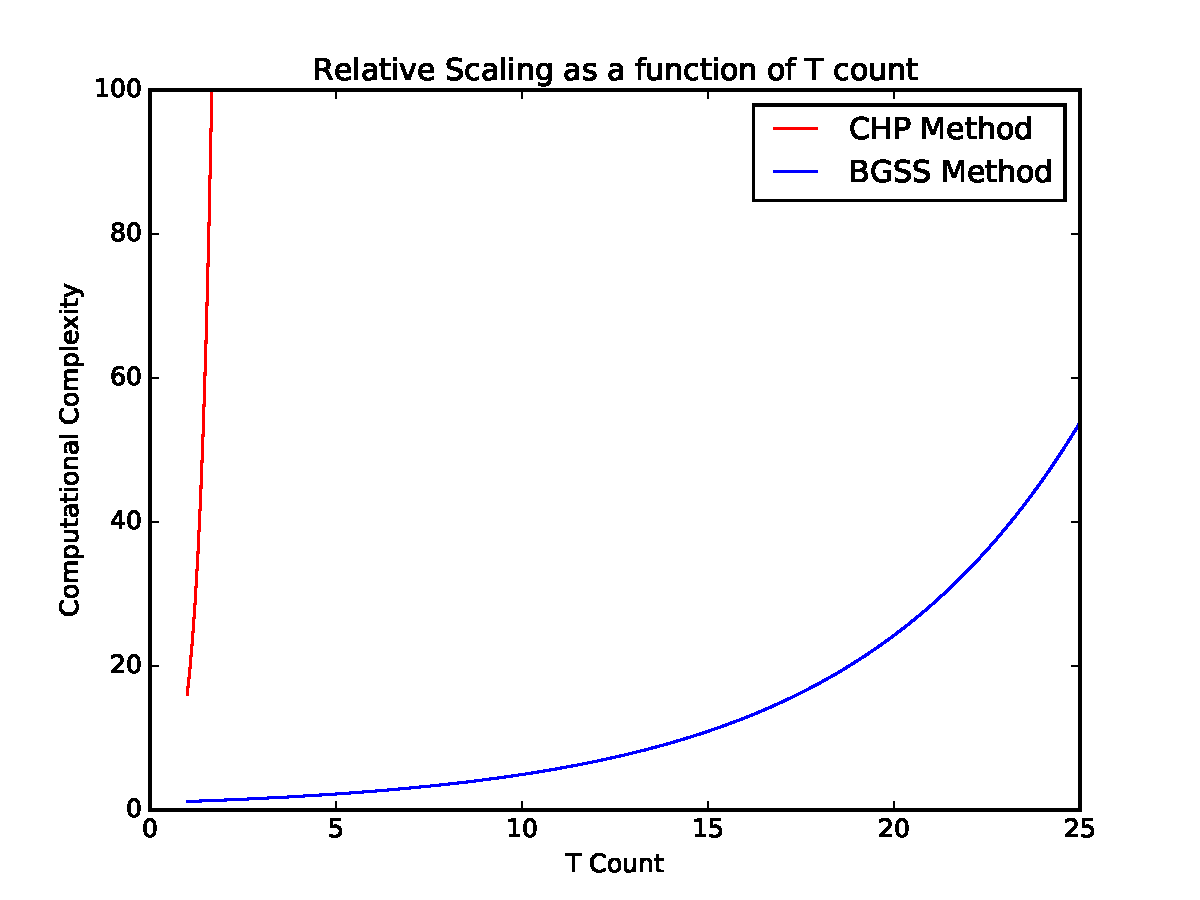
\includegraphics[width=0.6\textwidth]{Figures/tcount.pdf}
\label{fig:quadraticreduction}
\caption{Plot showing the relative behaviour of the dominant exponential scaling factors in the computational complexity for the \texttt{CHP} and \texttt{BGSS} algorithms, simulating a Clifford+T circuit.}
\end{figure}

\section{Significance for Quantum Computing}\label{sec:whybgss}
What Bravyi, Gosset, Smolin \& Smith have achieved is a significant reduction in the computational complexity needed to simulate a Clifford+T circuit. An example of the relative magnitude of this exponential scaling between the \texttt{CHP} and \texttt{BGSS} is shown in Fig~\ref{fig:quadraticreduction}. \\
The 8-fold quadratic reduction in the exponential scaling is an extremely significant improvement. The scaling remains exponential; we have not developed a method for efficiently simulating a quantum computation, but the circuits are significantly easier to simulate than might be expected. Indeed, a circuit with up to $50$ T-gates has been simulated using a laptop~\cite{Bravyi2015}, rather than High Performance Computing resources. 
\par
If we conceptualise quantum speedup as the regime where classical simulation becomes hard, this relative ease of simulation seems to suggest that the T gate has a limited computational power. This would imply we need to consume a large of magic states to realise a quantum algorithm which shows exponential speedup.\\
This indeed seems to be the case; using an implementation of a unitary synthesis algorithm for Clifford+T circuits, I obtained an estimate of 2000 $T$-gates required to realise Shor's algorithm on 10 qubits~\cite{Selinger2012}. Even with the significant reduction in complexity, this would be impractical to simulate using the \texttt{BSSG} method. 
\par
This suggests, then, that the Stabiliser Rank of a given state might instead serve as a useful measure of its value as a quantum computational resource. 

\section{Details of the Implementation}
\subsection{Representations of Stabiliser Groups}
\subsection{Computational Complexity}
\ifstandalone
\bibliography{../MResProject.bib,../ManualEntries.bib}
\fi
\end{document}
